Since we have closed form solutions for each parameter, we can estimate the parameters using the MLE from the real volatility data. The following section goes into the empirical modelling of the realised volatility through the estimation of each parameter of Ornestien-Uhlenbeck process. We select a cross-section of 100 tickers spread over 34 different asset classes or industry. See appendix for all the tickers.

\subsubsection{ Measurement of Realised Volatility}

We start with aggregated quote data over each 1-minute interval for each of the 100 tickers. Given an ask $A$ and a bid $B$, we calculate the weighted mid-price for each minute using the following formula.

$$
P_{\text{mid}} = A \cdot \frac{A_{\text{size}}}{A_{\text{size}} + B_{\text{size}}} + B \cdot \frac{B_{\text{size}}}{A_{\text{size}} + B_{\text{size}}}
$$

This 1-minute weighted mid price is now used to generate Open, High, Low, Close prices for each 5-minute interval. We construct 5 minute log-returns over these intervals. Suppose we have a price process $S_t$ and a time scale $\Delta$  the log returns $r_t$ are defined as:

$$	r_t = \log(S_t) - \log(S_{t-\Delta}) $$

The standard deviation of these 5-minute log-returns over a 6.5 hour trading day gives us a realized volatility estimate at a 5-minute resolution. There are twelve 5-minute intervals in an hour, there are 6.5 hours in a trading day and 252 trading days in a year. Therefore, this standard deviation is annualized by multiplying a constant = $\sqrt{12\times 6.5 \times 252}$.

\subsubsection{ Ambient Volatility $(\theta)$}

The following chart shows the long term  volatilities as estimated by Ornestein-Ulhenback process aggregated for each industry / asset class. This chart and other charts that will follow have been aggregated by the asset class reveals many interesting insights. However, it should be noted that the chart may not be truly representative because of the representation bias, as we have finite number of tickers representing each asset class. On the left end of the distribution are Agriculture and Crypto (spot) asset classes.  

\begin{figure}[H]
    \centering
    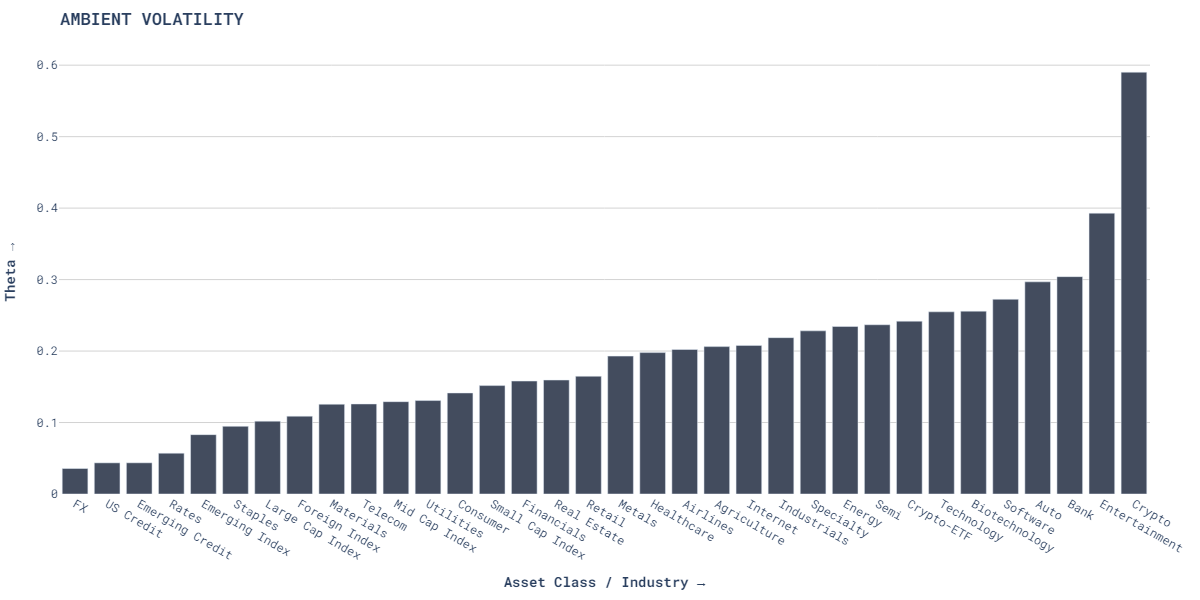
\includegraphics[width=\textwidth]{images/ambient_volatility_by_category.png}
    \caption{Ambient Volatility by Category}
    \label{fig:theta_by_category}
\end{figure}


The Cryptocurrencies which are deeply speculative in nature has an extraordinarily high ambient volatility compared to other asset classes. The entertainment industry which is mainly driven by consumer cyclicality seconds cryptocurrency in terms of long run volatility.
The sectors which are driven by innovation cycles and competitions such as technology biotechnology and automotive have relatively moderate ambient volatilities. The assets such as FX, Corporate and Treasury bonds  which are driven by macroeconomic factors such as interest rates, credit risks have the lowest levels of ambient volatility because their volatility are actively managed by central banks.


\subsubsection{ Mean Reversion $(\kappa)$}
The most interesting aspect of this kind of analysis is looking at the strength of mean reversion across tickers and asset classes.  The following chart shows the mean reversion rates as estimated by Ornestein-Ulhenback process aggregated for each sector. Although this chart is not very interpretable, therefore, in the next paragraph we modify the this mean reversion coefficient so as to look at expected time taken to reach the ambient volatility $(\theta)$ starting from a certain level of volatility. This helps to introduce interpretability in the mean reversion coefficient.

\begin{figure}[H]
    \centering
    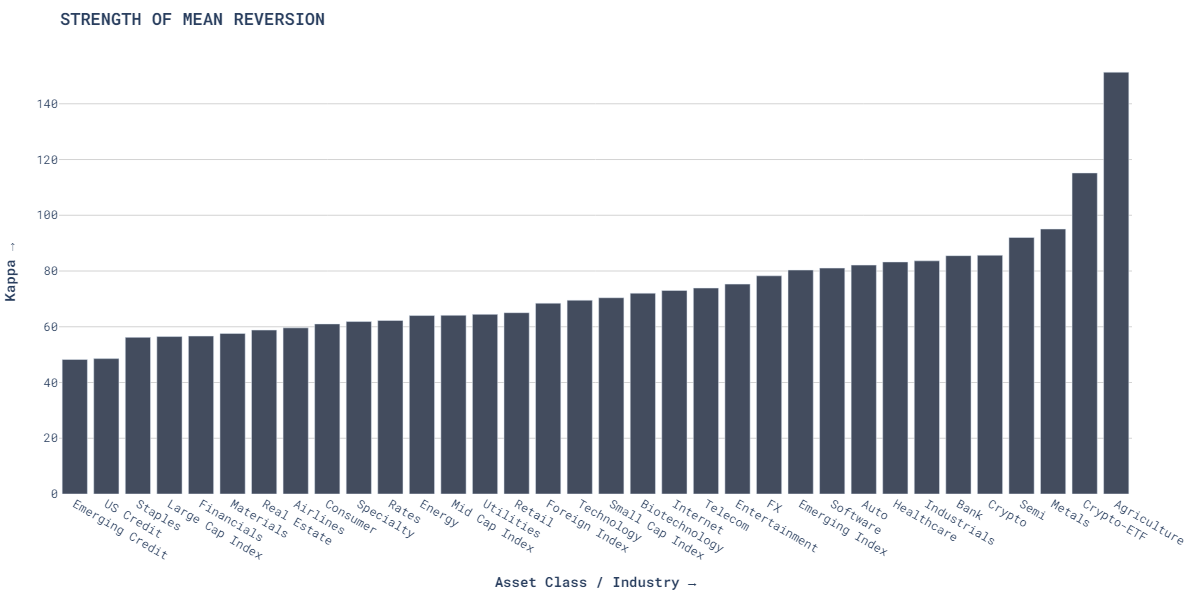
\includegraphics[width=\textwidth]{images/mean_reversion_by_category.png}
    \caption{Mean Reversion By Category}
    \label{fig:figure_label}
\end{figure}

Now since we know the mean reversion coefficient, we can ask another interesting question what is the expected amount of time it would take to reach from one level of volatility to another level of volatility. Since we have calibrated all the parameters of the stochastic differential equation, we can simulate different paths the volatility process could take which will enable us to look at the distribution of these Monte Carlo paths to estimate the parameter of interest.

To determine the expected amount of time that would elapse before the volatility touches its long run mean ($\theta$), we would first need to define, the first hitting or crossover time of the volatility process. Suppose we start from a volatility level $C$ and want to reach a volatility level of $A$. The expected time $T_{AC}$ can be expressed as an infimum over the set of all days $t$ where a single path crosses that volatility threshold.

$$ T_{A,C} = \inf\biggl\{ t\geq 0 \;: \; X_t = A \bigg| X_0 = C   \biggr\} $$

We can generate a large number of paths and the average of the infimums will give us the expected time to reach the level of ambient volatility.

To illustrate this concept, we can look at the iShares 20+ Year Treasury Bond ETF (TLT) which has a relatively slower mean reversion ($\kappa$) and we set the initial volatility level to be very high at 0.5, for the sake of a nice visualization. The estimated ambient volatility ($\theta$) of this ticker through Ornestien-Uhlenbeck process is 0.08. We generate 5000 Monte Carlo paths and we can observe that the volatility process is mean reverting to its ambient level over all the paths. To estimate the expected time to reach the ambient level, we take the average of the first crossovers over 5000 paths, which comes out to be 13.1 trading days with a standard error of 0.07 trading days.

\begin{figure}[H]
    \centering
    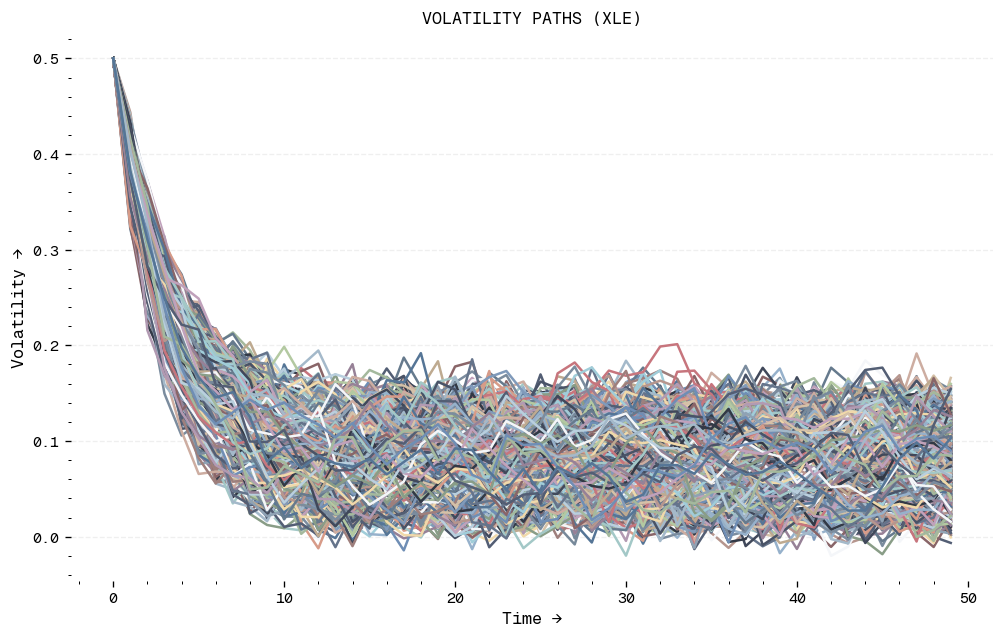
\includegraphics[width=\textwidth]{images/volatility_paths.png}
    \caption{Simulated 5000 paths of volatility process for TLT}
    \label{fig:figure_label}
\end{figure}

Please also note that very few volatility paths drop below zero. This is a Weiner process artefact and can be ignored, since we are looking at sufficiently large number of realizations.

A more interpretable version of looking at the mean reversion is to look at the expected number of days it will take for the volatility to reach its ambient level, given a starting level of volatility. The following chart shows the expected number of days it will take for the volatility to reach its ambient level ($\theta$) estimated through Ornestien-Uhlenbeck process for each industry / asset class, when we start from a pathologically high level of volatility of 0.5.

\begin{figure}[H]
    \centering
    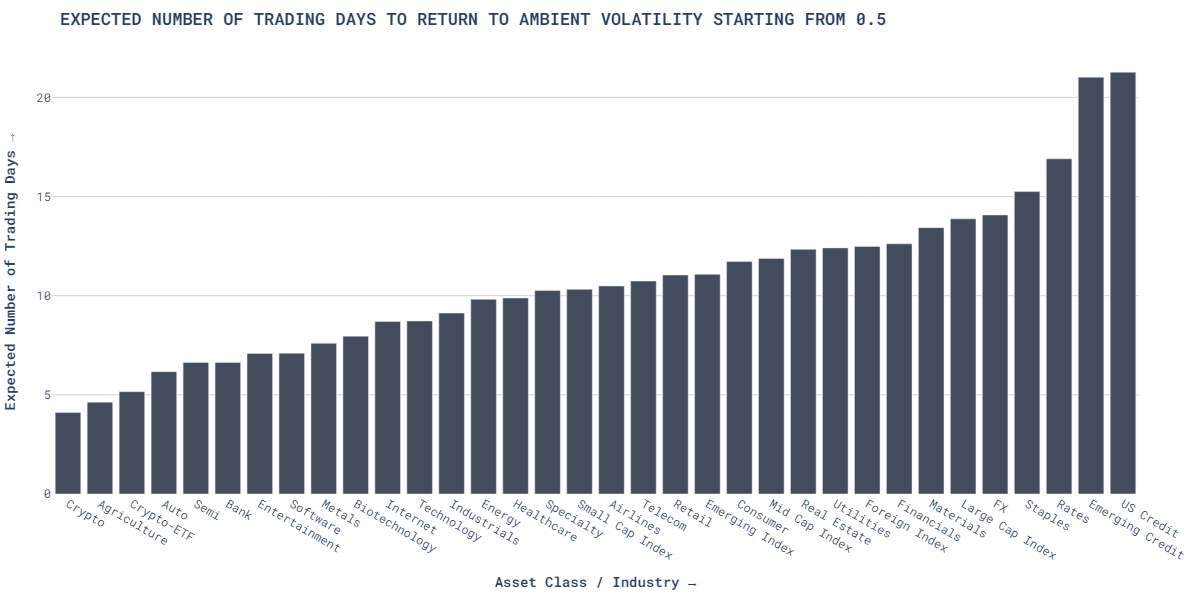
\includegraphics[width=\textwidth]{images/time_to_theta.png}
    \caption{Expected Time to Reach Ambient Volatility starting from a high volatility of 0.5}
    \label{fig:figure_label}
\end{figure}


If we start from a high volatility of 0.5, they take approximately four trading days to mean revert to their ambient volatility. A strong mean reversion tendency in agricultural tickers  is possibly due to the strong seasonal fluctuations inherent in these industries (\cite{Sorensen1999}). Cryptocurrency markets might be characterized by strong bursts of volatility which quickly stabilizes.

On the right end of the distribution, we have the industries that are highly sensitive to macroeconomic factors that influence credit markets such as Corporate bonds ETFs (HYG and LQD), Treasury Bond ETFs (TLT and IEF) of US and other emerging markets (EMB). These asset classes are heavily influenced by interest rates and default risks. Interest rate cycles usually span over several months and hence the volatility is expected to be persistent in these asset classes.

All the asset classes that relate to commodities and industrials like metal and energy sectors show reversion time around 6 to 8 trading days (starting from a high volatility) which indicates a relatively moderately persistent volatility.  The chart does not show the standard errors associated with each estimate of expected number of days however the standard error is extremely low possible because of a large sample realizations (5000 paths). The maximum standard error observed for the expected number of days over all tickers is one tenth of a trading day. The expected time levels as well as their associated standard errors for each ticker is shown in the appendix.

One more interesting insight emerges when we look at the scatter of the mean reversion against ambient volatility. 

\begin{figure}[H]
    \centering
    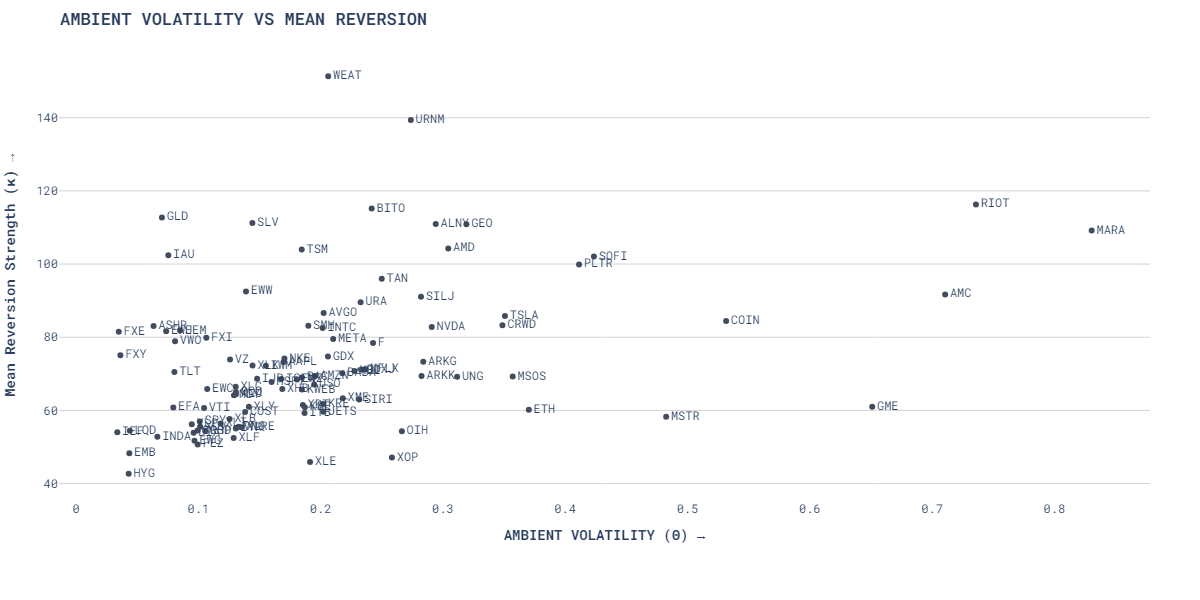
\includegraphics[width=\textwidth]{images/ambient_volatility_vs_mean_reversion.png}
    \caption{Scatter of Ambient Volatility vs Mean Reversion}
    \label{fig:figure_label}
\end{figure}

The strength of mean reversion has a heteroscedastic relationship with ambient volatility that is the variability of mean reversion across the cross section of tickers is conditional on what level of ambient volatility we are looking at.  At the lower levels of ambient volatility we find a strong visible correlation between the strength of mean reversion and ambient volatility which further dampens as we move to higher levels of ambient volatility across the cross section of tickers.



\subsubsection{ Meta Volatility $(\sigma)$  }

The meta volatility is the volatility of the volatility. The following chart shows the meta volatility as estimated by Ornestein-Ulhenback process aggregated for each industry / asset class.

\begin{figure}[H]
    \centering
    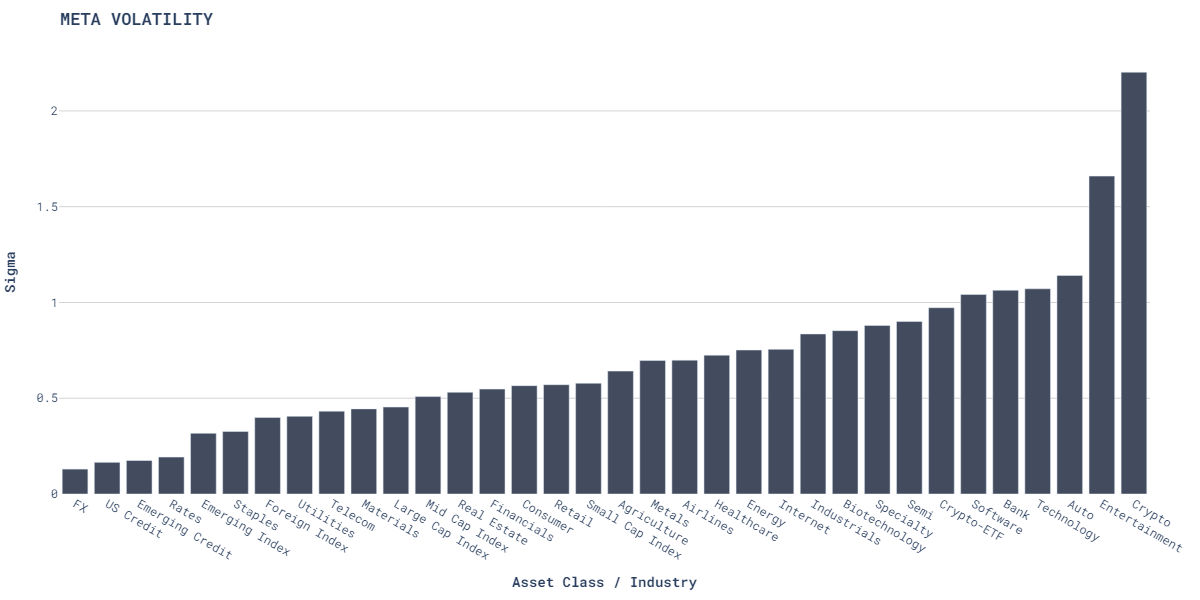
\includegraphics[width=\textwidth]{images/meta_volatility_by_category.png}
    \caption{Meta Volatility by Asset Class}
    \label{fig:figure_label}
\end{figure}

A truly interesting insight here is that this chart looks very similar to the ambient volatility chart in Figure \ref{fig:theta_by_category}. The empirical implication here is that if a asset class is characterized by a high level of ambient volatility, the volatility inherent in the ambient volatility is also high. This is apparently visible if we  look at the scatter of meta volatility against the ambient volatility.

\begin{figure}[H]
    \centering
    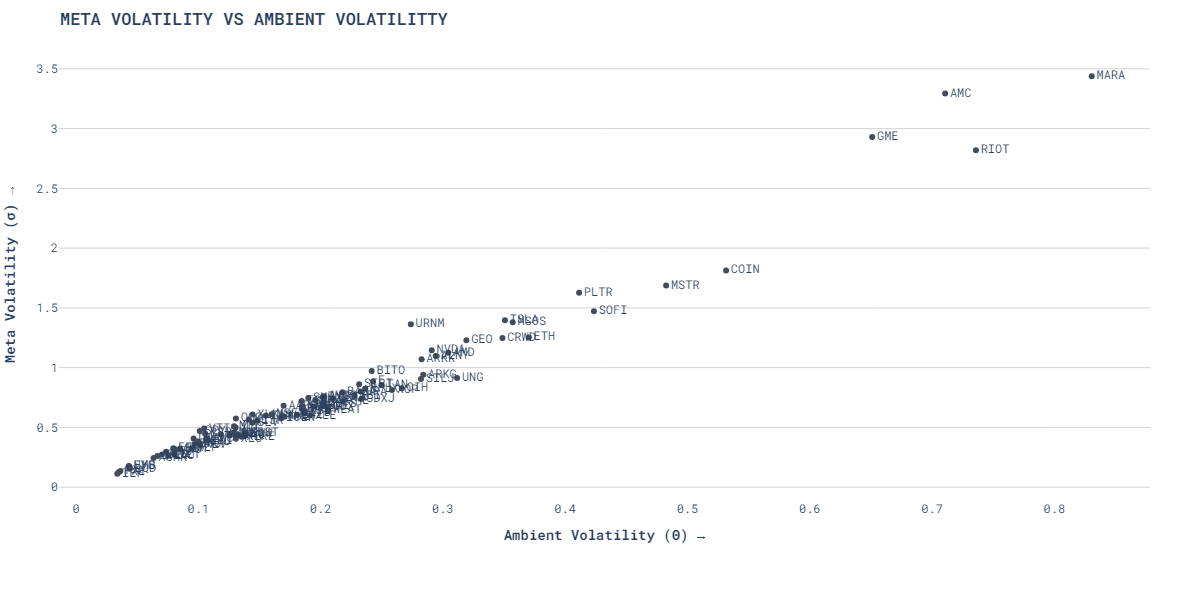
\includegraphics[width=\textwidth]{images/meta_volatility_vs_ambient_volatility.png}
    \caption{Scatter of Meta Volatility vs Ambient Volatility}
    \label{fig:figure_label}
\end{figure}

The relationship of meta volatility with the strength of mean reversion is similar to the relationship of ambient volatility with that of mean reversion. This is evident in the scatter below.

\begin{figure}[H]
    \centering
    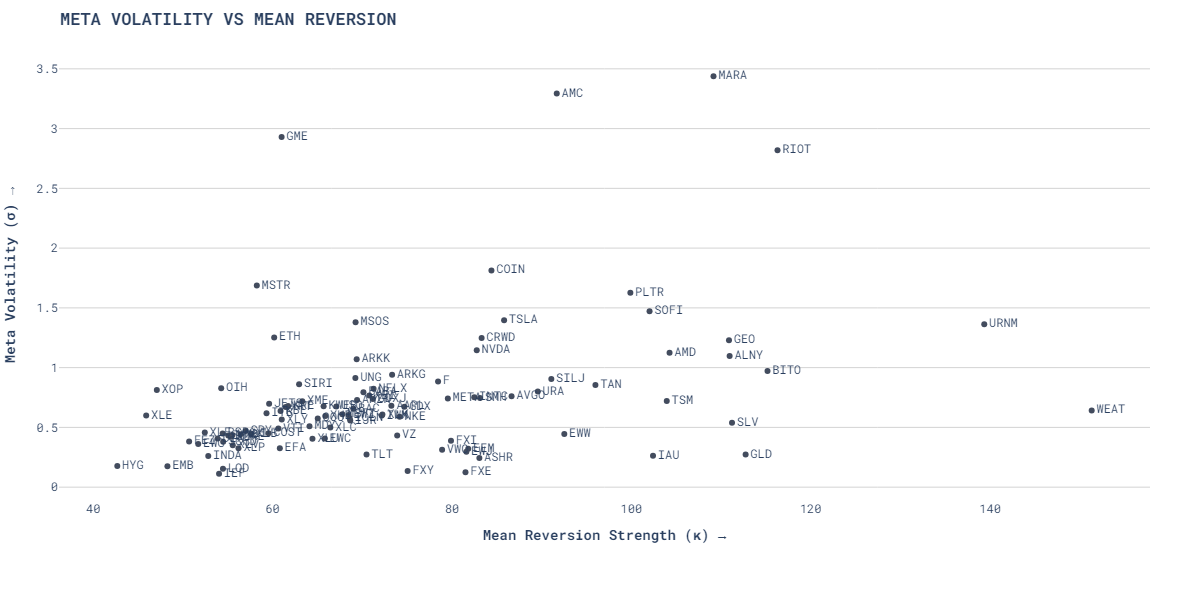
\includegraphics[width=\textwidth]{images/meta_volatility_vs_mean_reversion.png}
    \caption{Scatter of Meta Volatility vs Mean Reversion}
    \label{fig:figure_label}
\end{figure}

\section{ Roadmap from here}

\begin{displayquote}

“Forty-two!" yelled Loonquawl. "Is that all you've got to show for seven and a half million years' work?"  "I checked it very thoroughly," said the computer, "and that quite definitely is the answer. I think the problem, to be quite honest with you, is that you've never actually known what the question is.”  - Douglas Adams, The Hitchhiker’s Guide to the Galaxy

\end{displayquote}

Now I will venture into options market from the underlying spot markets.  The options market gives me two additional pieces of information that is the implied volatility and the skew.  At this point, I have a powerful model for the realised volatility.  This will enable me to ask good questions about  the implied volatility and the markup of the implied and the realised volatility that is the volatility risk premium.

\begin{enumerate}
\item Every trading day I can measure the distance between the realised volatility from the ambient volatility. The farther is the the realised volatility from the ambient volatility, it will be interesting to see how Volatility Risk Premium moves. Using these insights, can I find options that are mispriced or priced cheaply in the market?
\item I can use the gap between realised volatility and ambient volatility to see if market is overreacting to short term volatility bursts. This could be an incredibly useful trading signal.
\item Is the current implied volatility accurately pricing the future realized volatility? Is there a pattern when implied volatility consistently overshoots or underpredicts the future realised volatility.
\item I also know the mean reversion speed of the volatility process for each ticker. This can reveal potential mispricing of short term options.
\item How does the skew move with realized volatility?
\item How is skew distributed across asset classes?
\end{enumerate}


These questions would change and evolve as I move forward in the thesis. I am not sure, if I am still asking the right questions. The questions would themselves appear with the data. Motion creates information. Peace.

